\section{A calibration workflow and reproducible examples}\label{sec:calibration}
\subsection{What to collect and what to report}
A single cross-section suffices for a calibration illustration. It does not suffice to establish stability through time, estimate a physical risk premium, or compare hedging performance. For the cross-section, collect settlement date, exact option expiry, option type, strike, settlement premium, underlying futures identifier and settlement, and the underlying accrual start and end dates. Retain volume or open interest as context, rather than interpreting their presence as proof that a settlement is an executable quote. Add the meeting schedule and, for discounted cash pricing, the discount curve.

The following workflow implements the distinction between fit and identification.
\begin{enumerate}
\item \emph{Map contracts before fitting.} Serial options and quarterly options can reference the same underlying future. The option month is not its accrual window. Convert all premiums to one rate unit and use a consistent day count. Listed futures options use a price index that falls as the implied rate rises; a call on that index corresponds to a put on the rate after changing the strike and scale.
\item \emph{Specify the pricing experiment.} State whether the pricer treats European cash exercise or the actual listed exercise convention. State the assumed background variance schedule and maturity loadings. List any parameters imported from historical estimation.
\item \emph{Extract a small set of price quantities.} Fit the surface parameters $(D,m,q)$, or bound them over acceptable price errors. Inspect variation of implied variance across strikes. Under the Gaussian specification, systematic smile residuals indicate misspecification.
\item \emph{Construct the observation matrix.} Use the actual observed expiries and windows, compute its rank, and identify its row space. Add futures-assisted rows only if their price uncertainty is also retained.
\item \emph{Fit and bound.} Report a nonnegative fit and the extrema of individual variances and relevant group totals over the feasible set. Repeat under specified price tolerances and a small number of economically distinct background assumptions.
\item \emph{Check omitted prices and disclose failure.} Compare with strikes or expiries excluded from calibration. If no parameter vector fits the enlarged set at the stated tolerance, report that fact separately from the ranges obtained using the calibration subset.
\end{enumerate}
Historical bid--ask data are not an input to these steps. If current executable quotes are available, their spreads can inform the price intervals. With settlements alone, use disclosed tolerance scenarios. An interval of one or two settlement increments is an assumption about acceptable price error, not an estimate of a historical spread, transaction cost, or confidence level.

\subsection{A controlled variance-panel precision example}\label{sec:synthetic}
Take five meetings spaced $0.10$ year apart, from $0.10$ through $0.50$. Observe six option expiries spaced $0.10$ year apart, from $0.05$ through $0.55$. All options refer to the accrual window $[1,1.25]$. Each meeting has variance $100$ bp$^2$, and the constant background variance rate is $2{,}500$ bp$^2$ per year. The initial forward curve is flat at $4\%$. The first gap contains no meeting and each later gap contains exactly one, so Theorem~\ref{thm:rank} gives exact identification of all six parameters.

Generate the European prices from Proposition~\ref{prop:pricing}. For this controlled precision experiment, keep each discount factor and forward-measure mean fixed at its model value and use a strike equal to that mean. This fixes the nonlinear price-to-variance conversion while isolating uncertainty in the variance panel. We deliberately do not impose the additional model equations linking those means to the candidate variances and futures prices. The exercise is therefore an exact calculation for the extracted variance intervals, rather than a joint recalibration of every generated price. The generated cumulative variances are $125,475,825,1175,1525,1875$ bp$^2$. Invert premium intervals exactly by \eqref{eq:inverse}, and solve \eqref{eq:LP} for each meeting variance and the background rate.

Figure~\ref{fig:precision} shows the resulting sharp variance-panel ranges at premium tolerances of $0.25$ and $0.5$ rate basis points. At $0.25$ bp, the first meeting range is $[30.3,168.1]$ bp$^2$, while the fifth is $[0,231.3]$ bp$^2$. At $0.5$ bp, all five individual ranges include zero. Although every meeting is isolated by an expiry, finite price precision leaves wide intervals around the true value of $100$ bp$^2$. Later intervals are affected by the larger total accumulated uncertainty. The uncertainty in the background, learned from a short first gap, also propagates into every meeting estimate.

\begin{figure}[ht]
\centering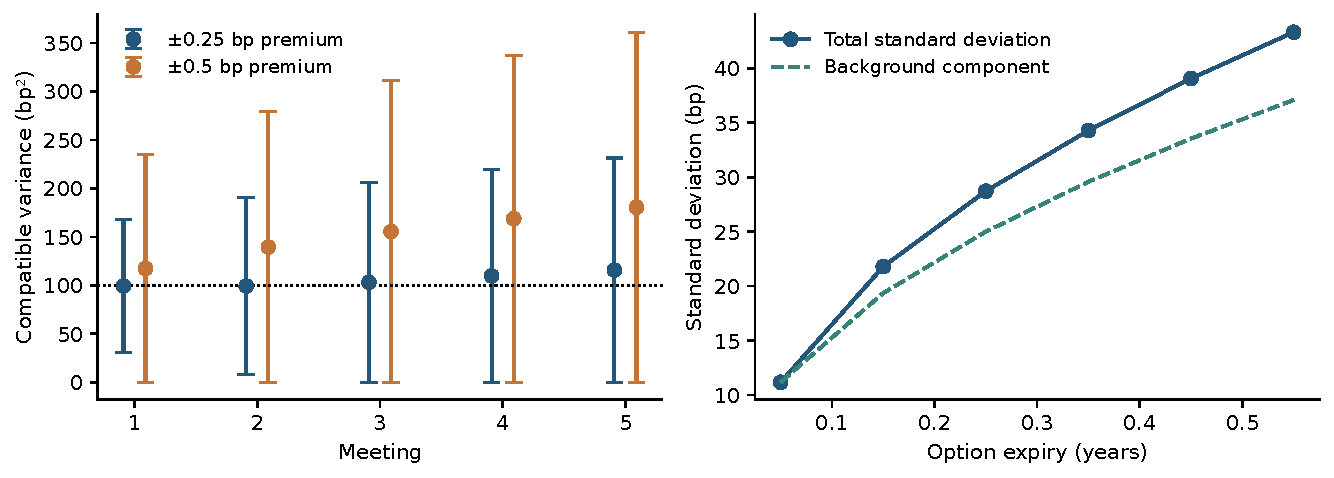
\includegraphics[width=.96\textwidth]{figures/precision.pdf}
\caption{Synthetic European variance-panel example. Left: sharp individual meeting-variance ranges for the extracted variance intervals, using fixed option means and discount factors for inversion; the dotted line is the true variance. Right: accumulated standard deviation and its background component. Full rank does not imply narrow ranges at finite price precision.}\label{fig:precision}
\end{figure}

All inputs and endpoint calculations are generated by the accompanying script. No simulation error enters this example. The price intervals are deterministic perturbation sets; they do not purport to contain a true parameter with a specified probability.


The next section applies the same sequence---contract mapping, fit checks, and feasible ranges---to a historical settlement panel. Section~\ref{sec:uses} then considers how those outputs can inform relative-value screening and hedge construction.
